\section{Technology Stack and Design Rationale}
The selection of the technology stack is predicated on achieving a highly scalable, maintainable, and secure platform, particularly critical for handling sensitive medical imaging data. This section justifies the architectural philosophy and the specific technologies chosen for each layer of the system.

\subsection{Architectural Philosophy}
The platform adopts a decoupled, multi-tiered architecture comprising a PostgreSQL-centric backend and a modern React frontend. This architectural philosophy is a strategic choice to ensure robust scalability, enhanced maintainability, and clear separation of concerns. By decoupling the frontend (user interface) from the backend (business logic and data storage), each layer can be developed, deployed, and scaled independently, optimizing resource utilization and facilitating parallel development. The backend, centered around PostgreSQL, provides a reliable and extensible data foundation, while the React frontend offers a highly responsive and modular user experience. This modularity simplifies debugging, updates, and the integration of new features or technologies without extensive rework, thereby enhancing the system's long-term viability and adaptability.

The following diagram provides a high-level overview of the platform's architectural components and their interconnections, illustrating the decoupled nature of the system and the flow of data between the user, frontend, backend, and external medical imaging/AI services.

\begin{figure}
    \centering
    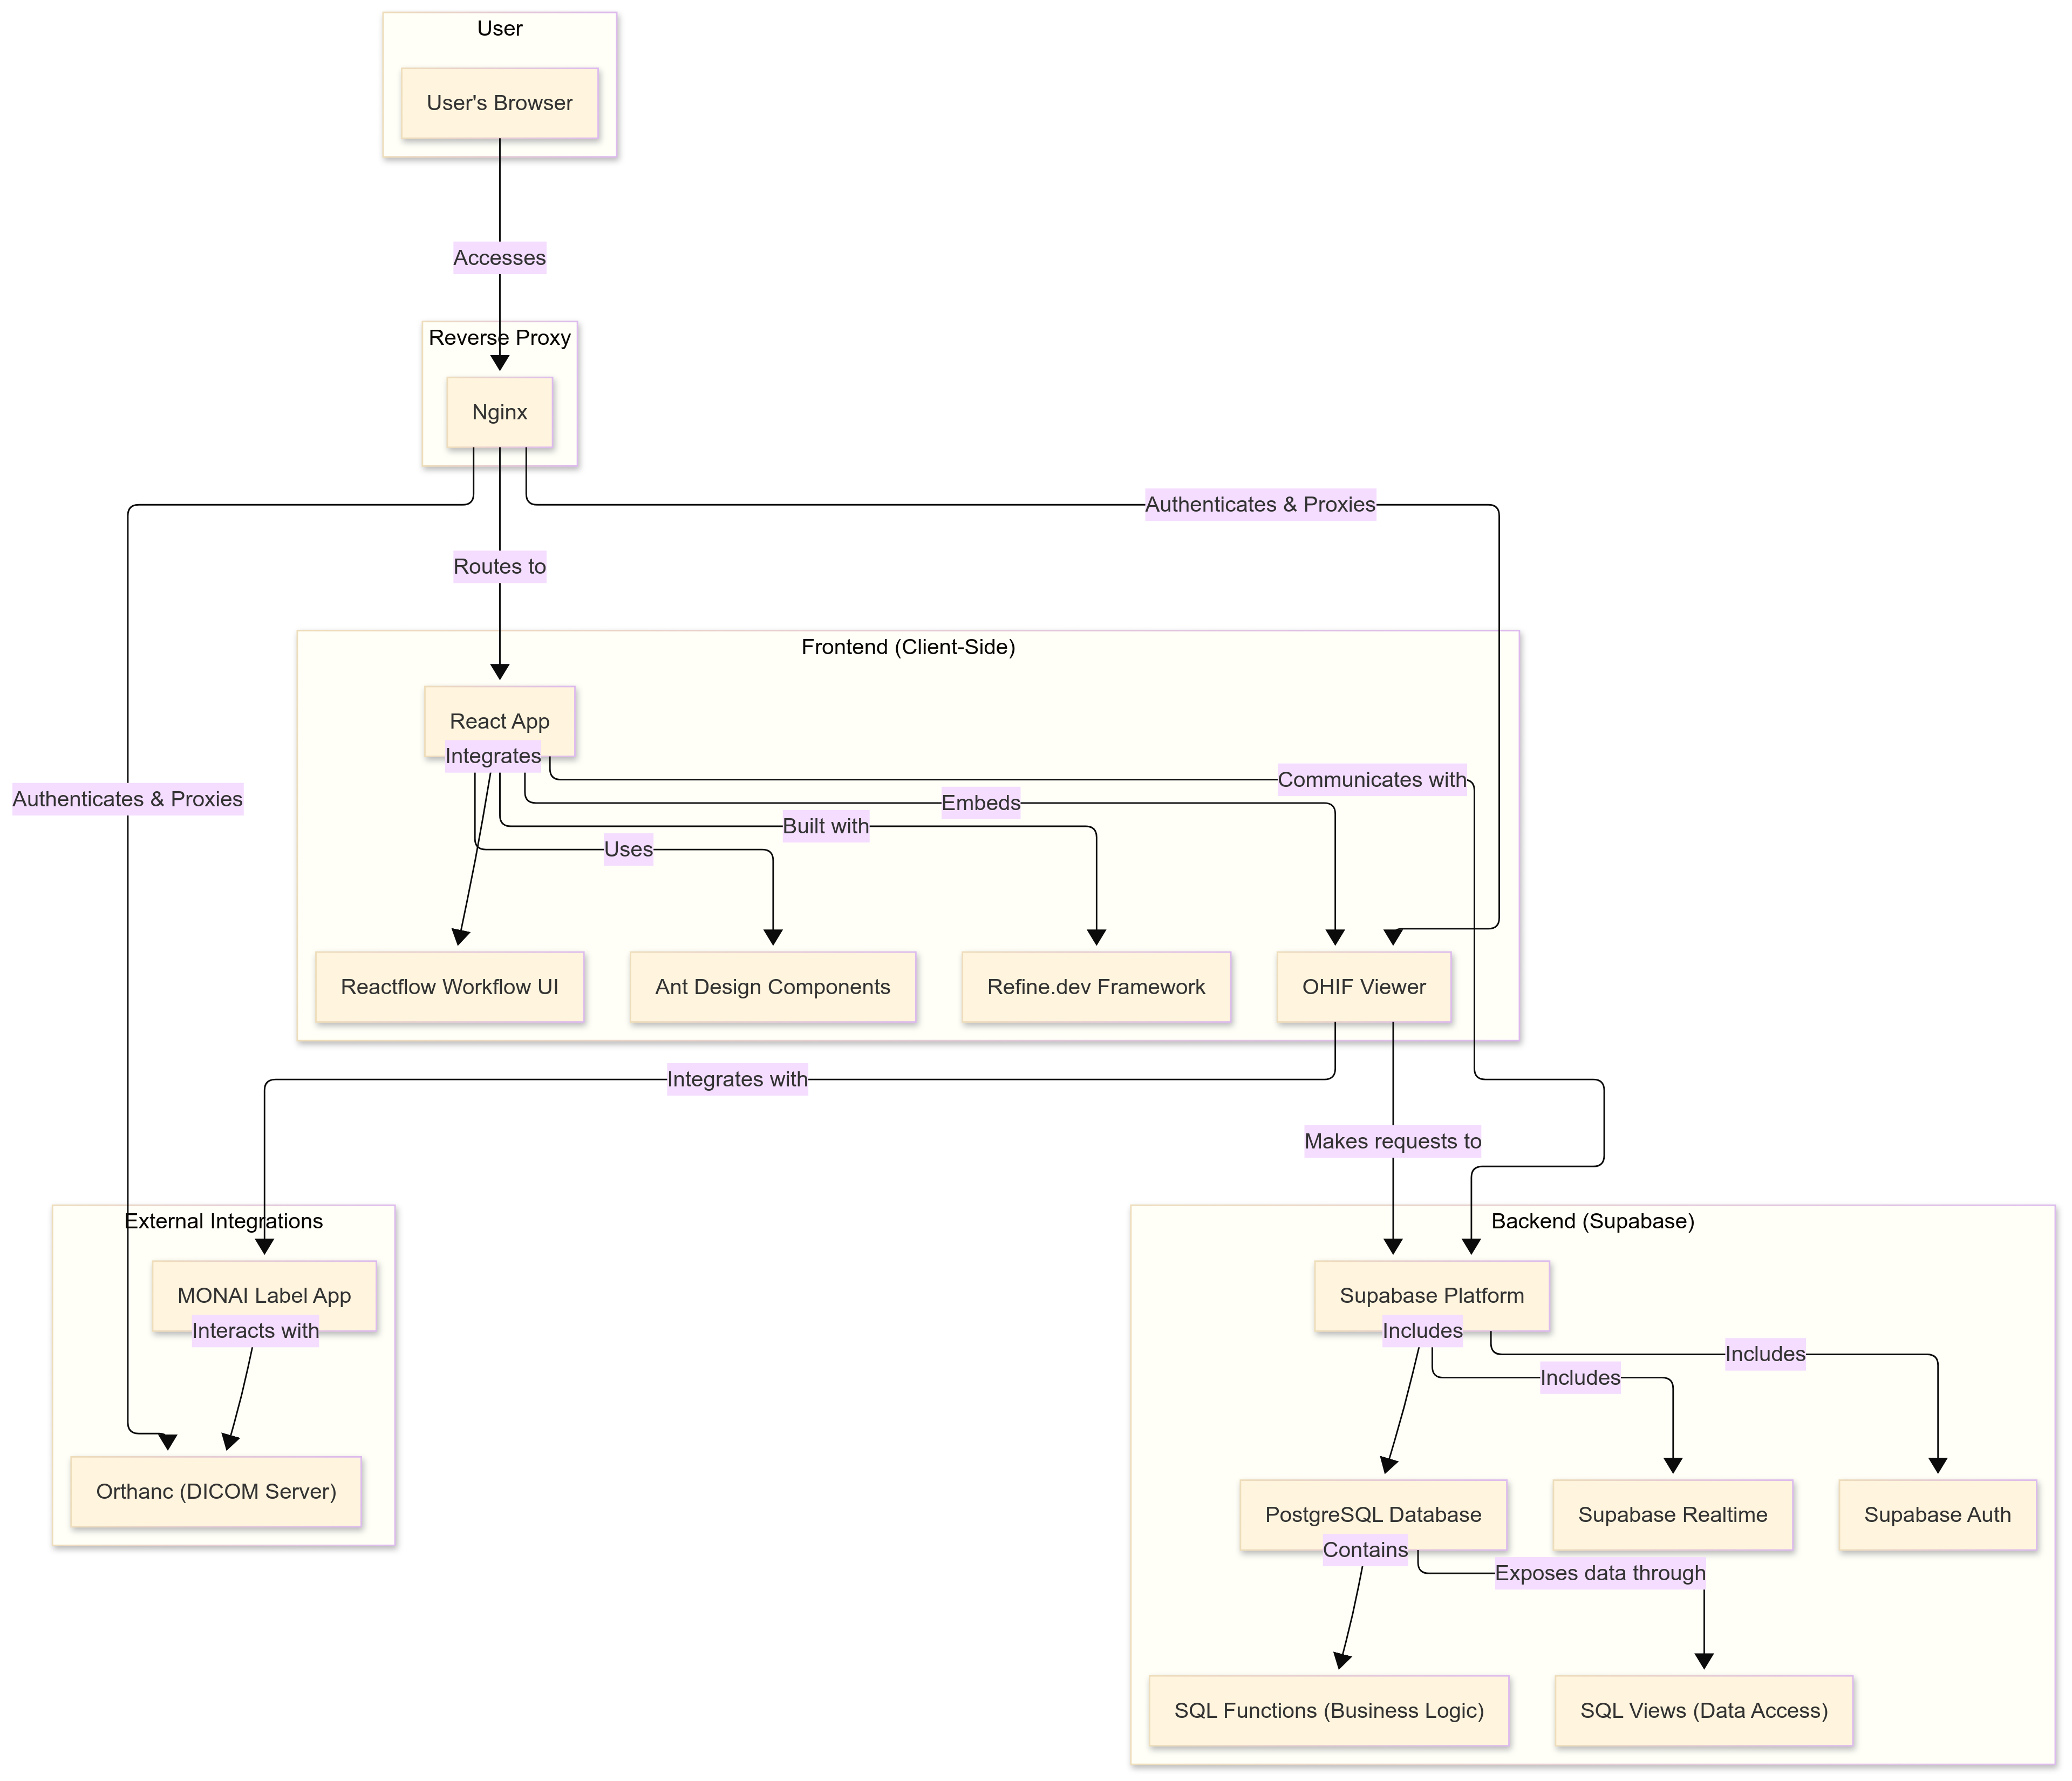
\includegraphics[width=1\linewidth]{content//resources//architecture.png}
    \caption{Overview of the platform's architecture}
    \label{fig:enter-label}
\end{figure}

\subsection{Frontend Rationale (React \& Refine.dev)}
The frontend is built with React, a leading JavaScript library renowned for its component-based architecture and declarative nature. React's component model promotes reusability, modularity, and maintainability, allowing complex UIs to be efficiently assembled from smaller, independent units. This facilitates parallel development and ensures a consistent design language across the application. React is a highly popular choice, running on 4.8\% of websites globally and being leveraged by approximately 41.6\% of professional developers according to a 2024 StackOverflow report. Its component architecture is reported to produce 60\% faster development times compared to monolithic architectures, and React-built sites can render 15-20\% faster than other JavaScript library-based websites. 

To accelerate development and provide enterprise-level features, the platform leverages Refine.dev. Refine is a headless frontend framework that streamlines the creation of data-intensive applications like admin panels and dashboards. It offers pre-built components and hooks for common enterprise functionalities, including CRUD (Create, Read, Update, Delete) operations, robust authentication flows, and flexible routing, significantly reducing boilerplate code and development time. Refine's backend-agnostic nature ensures compatibility with the chosen Supabase backend, providing 100\% control over the project without workflow constraints. Refine.dev is noted for its ability to significantly increase development speed, allowing data-heavy apps to be set up in a short amount of time, often less than a minute using its CLI. It boasts a community of 32K+ active developers and is used in 8K+ production projects. 

For a comprehensive and consistent user interface, Ant Design is integrated. Ant Design is a widely adopted UI library that provides a rich collection of high-quality, customizable, and accessibility-compliant React components. Its adherence to a unified design language ensures a cohesive look and feel across the application, improving team collaboration and reducing design-to-development discrepancies.

Finally, Vite is employed as the build tool and development server. Vite offers significantly faster development experiences due to its instant server start, lightning-fast Hot Module Replacement (HMR), and efficient production builds. It leverages native ES modules for on-demand file serving, eliminating the need for bundling during development, and performs optimized builds with Rollup for production, including code splitting and tree shaking for smaller bundle sizes and faster load times. 

\subsection{Backend Rationale (Supabase \& PostgreSQL)}
The backend is architected around Supabase, an open-source Backend-as-a-Service (BaaS) platform that provides a managed PostgreSQL database, authentication, real-time capabilities, and serverless functions. Supabase was chosen as a robust alternative to traditional backend development, simplifying much of the heavy lifting while offering the flexibility and transparency of open-source tools. 

At its core, Supabase utilizes PostgreSQL, a highly reliable, extensible, and performant relational database system. PostgreSQL is a dominant force in the relational database market, holding a 16.85\% share as of 2025, making it the second most used open-source database after MySQL. It is also recognized as the

most admired and desired database in recent surveys. This choice allows the platform to leverage the full power of SQL, including advanced queries, JSON support, and ACID compliance, ensuring strong data integrity and transactional consistency. In performance comparisons, PostgreSQL within Supabase demonstrates significant advantages for complex queries, with complex joins completing in 89ms compared to Firebase's 251ms, and aggregations in 103ms versus Firebase's 327ms. 

A key architectural strategy is the embedding of core business logic directly within PostgreSQL functions and triggers. This approach ensures atomicity and data integrity by executing logic directly at the database level, guaranteeing that operations are either fully completed or entirely rolled back. Triggers automatically execute SQL functions on table events (e.g., INSERT, UPDATE, DELETE), providing a powerful mechanism for enforcing business rules and maintaining data consistency directly within the database. While this approach can introduce challenges in debugging and potential vendor lock-in if overused , for critical business logic requiring high transactional integrity and direct data manipulation, it offers unparalleled reliability. 

\subsection{Medical Imaging \& AI Rationale (Orthanc, OHIF, MONAI)}
The selection of specialized tools for medical imaging and AI is crucial for addressing the domain-specific complexities and regulatory requirements.

\begin{itemize}
    \item \textbf{Orthanc}: Chosen as a lightweight, open-source DICOM server (mini-PACS). Orthanc simplifies the management and exchange of medical images by providing a modern RESTful API and full support for the DICOMweb standard (QIDO-RS, WADO-RS, STOW-RS). Its design abstracts the inherent complexity of the DICOM format and protocol, allowing developers to interact with medical images with minimal DICOM knowledge. This significantly reduces development overhead and accelerates the integration of medical imaging data into the web-based platform. Orthanc is noted for its lightweight nature and ability to run on standard desktop computers, making deployment almost immediate.
    \item \textbf{OHIF Viewer}: Selected as a powerful, open-source, web-based medical imaging viewer. OHIF is designed for rapid loading and visualization of large radiology studies, leveraging Cornerstone3D for efficient rendering and annotation. Its React-based, component-driven architecture and flexible plugin framework allow for seamless embedding and customization within the platform's frontend. OHIF's out-of-the-box compatibility with DICOMweb archives like Orthanc further streamlines data access. While a large study of 2500 instances (800MB) can take approximately 30 seconds to display in the viewport , OHIF is continuously optimized for performance, including GPU acceleration and multi-threading for quick image decoding.
    \item \textbf{MONAI}: Utilized as a standardized, open-source framework for medical AI. MONAI Label, a component of MONAI, provides intelligent image labeling and learning tools that enable AI-assisted annotation, active learning, and continuous model improvement specifically for medical images. Its support for state-of-the-art models and integration capabilities with viewers like OHIF make it an indispensable component for building powerful, integrated medical AI workflows. MONAI Label is reported to enable 50-80\% faster annotation time and 2x faster model convergence. The MONAI ecosystem has seen significant adoption, with over 3.5 million downloads and contributions from 220 individuals globally, and has been acknowledged in over 3,000 publications.
\end{itemize}

This integrated system—Orthanc for data management, OHIF for visualization and annotation, and MONAI for AI-driven assistance—forms a modular and powerful ecosystem tailored for medical imaging data annotation, ensuring compliance, efficiency, and advanced AI capabilities. 

\subsection{Infrastructure Rationale (Nginx, Azure, Cloudflare)}
The infrastructure design prioritizes security, performance, and ease of deployment.

\begin{itemize}
    \item \textbf{Nginx}: Employed as a reverse proxy to manage and secure traffic to all backend services. Nginx sits in front of the backend servers, distributing client requests, performing load balancing, and acting as an additional layer of defense against security attacks. It centralizes SSL/TLS termination, compresses data, and caches content, thereby offloading work from backend servers and improving overall performance and security. Its role simplifies network configuration and enhances the anonymity of backend services. Nginx has seen a significant rise in popularity, surpassing Apache in market share, reaching 34.1\% by November 2023 and 33.8\% of all websites whose web server is known as of July 2025.
    \item \textbf{Azure VM}: Chosen for hosting stateful backend services, specifically Orthanc and MONAI. Azure Virtual Machines provide the necessary computational resources, persistent storage, and network configurations required for these services, which often demand dedicated resources and specific environments for optimal performance and data residency. This ensures full control over sensitive medical data, allowing deployment within a secure, on-premise or private cloud infrastructure to meet stringent data privacy and compliance requirements (e.g., HIPAA, GDPR).
    \item \textbf{Cloudflare Pages}: Utilized for deploying the frontend application with integrated CI/CD capabilities. Cloudflare Pages is a JAMstack platform designed for static websites and dynamic frontends built with frameworks like React. It offers easy setup by integrating with GitHub/GitLab repositories, providing automatic deployments on code pushes, a global CDN for low-latency responses, and built-in SSL certificates. This choice ensures rapid deployment, global accessibility, and efficient content delivery for the user-facing application. Cloudflare's global network caches static content within 50ms of 95\% of all Internet users, and its CDN can provide a 1900ms (nearly 2 second) improvement in load time for static content by reducing the physical distance between the client and the data.
\end{itemize}

